\documentclass[]{article}
\usepackage[spanish]{babel} 
\usepackage{amsmath} 
\usepackage[colorlinks=true]{hyperref}
\usepackage{enumitem} 
\usepackage{graphicx}   
\usepackage[a4paper,top=2.5cm,bottom=2.5cm,left=2cm,right=2.5cm]{geometry} 
\usepackage[]{subfigure}
\usepackage[]{multicol}
\setlength{\columnsep}{1cm}
\usepackage[]{hyperref}
%\usepackage[maxbibnames=99, sorting=none]{biblatex}
\usepackage{amssymb}
\usepackage[]{txfonts}

%\usepackage[authoryear]{natbib}
\newenvironment{Figura}
  {\par\medskip\noindent\minipage{\linewidth}}
  {\endminipage\par\medskip}

\graphicspath{ {./imag/Lab-Termo/Git/Documentos}} 
\title{Jaula de Faraday} 
\author{Noemi de la Peña, Benjamín Opazo, Martina Contreras \\ \\
 \textit{ Departamento de Física, Universidad de Concepción, Concepción, Chile. }}
  \date{} 

  



   %==================================================================================
\begin{document}
\maketitle 



    


%=============Resumen============
\begin{abstract}
En este presente documento se expone una serie de datos y concluciones 
obtenidas a través de 3 experiencias de laboratorio. Relacionados con conceptos vistos en clases como: el campo electrico,
conductores y ondas electromagnéticas.
\end{abstract}

\begin{multicols*}{2}

%========Introducción=============
\section*{Introdución}
A medida que el saber del humano crece, también lo hace las preguntas.
¿Por qué al frotar un globo sobre mi cabeza los pelos se levantan? o 
<<<<<<< HEAD
¿Por qué al interior de una Capula de metal nuestro teléfonos pierden la señal?
Los antiguos griegos dieron hincapié al estudio de la ciencia que 
lograría dar respuesta a las anteriores interrogantes, El electromagnetismo.
Por medio de esta rama de la física, analizaremos 3 diferentes experimentos, donde describiremos el procedimiento y materiales a utilizar, además   formularemos nuestras conclusiones al final de este informe.

%==============Marco teorico============
\section*{Marco teorico}
Antecedentes históricos:
El electromagnetismo es la rama de la física que estudia las relaciones entre los fenómenos eléctricos y magnéticos, es decir, las interacciones entre las partículas cargadas y los campos eléctricos y magnéticos.
En 1821 los fundamentos del electromagnetismo fueron dados a conocer con el trabajo científico del británico Michael Faraday, lo que dio origen a esta disciplina. En 1865 el escocés James Clerk Maxwell formuló las cuatro “ecuaciones de Maxwell” que describen por completo los fenómenos electromagnéticos.
Michael Faraday , además  observó que un material conductor mostraba los efectos de una descarga eléctrica únicamente en su exterior. Esto parecía indicar que las cargas del conductor se distribuían de tal manera que cancelaban los campos eléctricos internos.
Este descubrimiento daría idea a la jaula de Faraday, la cual es un contenedor recubierto con materiales conductores de electricidad que funciona como blindaje contra los efectos de los campos eléctricos
=======
¿Por qué al interior de una Capula de metal nuestro teléfonos pierden la señal ?
Los antiguos griegos dieron hincapié al estudio de la ciencia que 
lograría dar respuesta a las anteriores interrogantes, El electromagnetismo.
Por medio de esta rama de la física, analizaremos 3 diferentes experimentos, donde describiremos el procedimiento y materiales a utilizar, además   formularemos nuestras conclusiones al final de este informe.

%

%==============Marco teorico============
Antecedentes históricos:
El electromagnetismo es la rama de la física que estudia las relaciones entre los fenómenos eléctricos y magnéticos, es decir, las interacciones entre las partículas cargadas y los campos eléctricos y magnéticos.
En 1821 los fundamentos del electromagnetismo fueron dados a conocer con el trabajo científico del británico Michael Faraday, lo que dio origen a esta disciplina. En 1865 el escocés James Clerk Maxwell formuló las cuatro “ecuaciones de Maxwell” que describen por completo los fenómenos electromagnéticos \cite{electromagnetismo}.
Michael Faraday , además  observó que un material conductor mostraba los efectos de una descarga eléctrica únicamente en su exterior. Esto parecía indicar que las cargas del conductor se distribuían de tal manera que cancelaban los campos eléctricos internos.
Este descubrimiento daría idea a la jaula de Faraday, la cual es un contenedor recubierto con materiales conductores de electricidad que funciona como blindaje contra los efectos de los campos eléctricos \cite{Jaula de Faraday}
>>>>>>> 8e44a590e3c470e181ed38a81a57aefe5d0abf0c
Palabras claves: Campo eléctricos, electromagnetismo, conductores y jaula de Faraday. 


%========Objetivos==================
%\section{Objetivos}



%=========Materiales===============
\section*{Materiales}

\begin{multicols*}{2}
\begin{itemize}
    \item celular
    \item papel de aluminio
    \item jabón
    \item agua
    \item globo
    \item bombilla
    \item bolsa ziploc
    \item audífonos
    \item colador de metal 
\end{itemize}
\end{multicols*}




%================Procedimiento=================================
\section*{Experimento 1}
\textit{Materiales: Papel de aluminio, celular.}

\vspace{-\topsep}
\begin{itemize}
    \setlength{\parskip}{0pt} 
    \setlength{\itemsep}{0pt plus 1pt}
    \item Primero, ponemos el celular sobre el papel de aluminio.
    \item Segundo, desde otro móvil, llamamos al celular del experimento para comprobar que funciona correctamente.
    \item Luego envolvemos el celular con el papel de aluminio.
    \item Finalmente volvemos a llamar, y notamos que el celular no recibe las llamadas.
\end{itemize}
\vspace{-\topsep}


\begin{Figura}
    \centering
    \includegraphics[width=2cm, height=3cm]{imag/Exp1_00.jpg}
    \includegraphics[width=2cm, height=3cm]{imag/Exp1_01.jpg}
    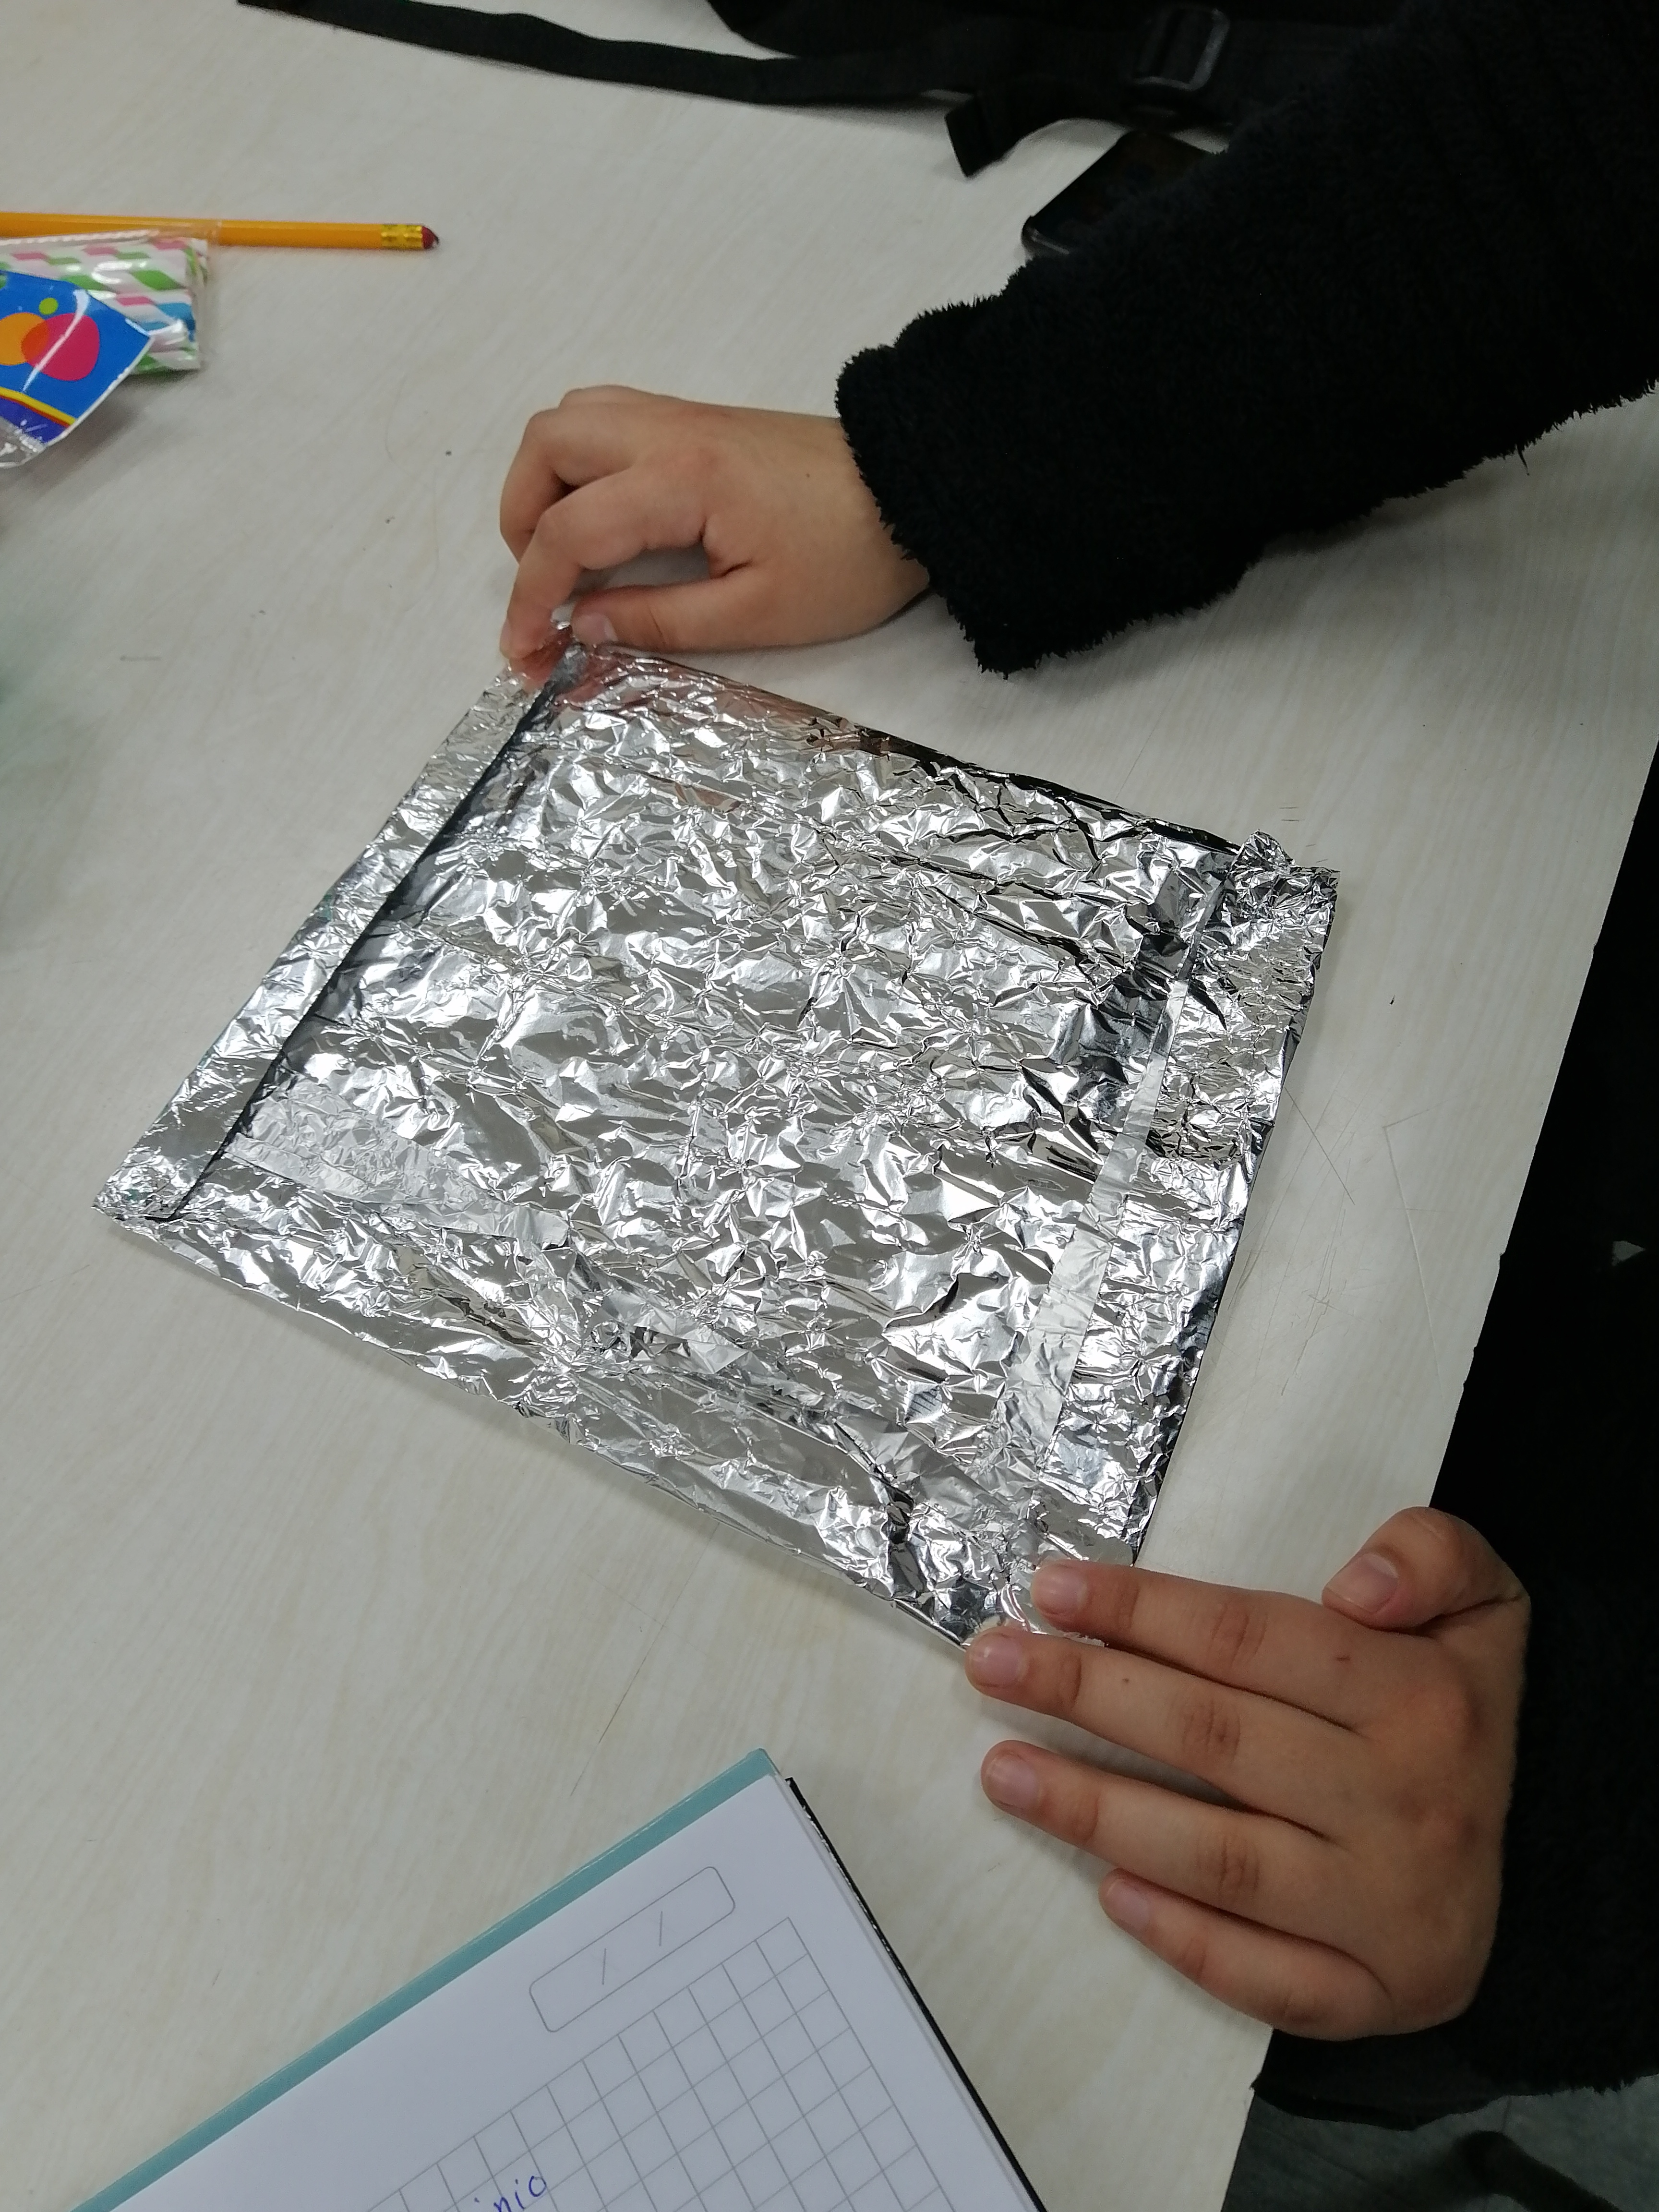
\includegraphics[width=2cm, height=3cm]{imag/Exp1_02.jpg}
\end{Figura}

%%%%%%%%%%%%%%%%%%%%%%%%%%%%%%%%%%%%%%%%%%%%%%%%%%%%%%%%%%




\section*{Experimento 2}
\textit{Materiales: Jabón, agua, bombilla, globo, bolsa ziploc.}

\vspace{-\topsep}
\begin{itemize}
    \setlength{\parskip}{0pt} 
    \setlength{\itemsep}{0pt plus 1pt}
    \item Primero mezclamos el agua con el jabón.
    \item Segundo, sobre la bolsa ziploc, desparramamos un poco de la mezcla hecha anteriormente.
    \item Después inflamos el globo y lo frotamos contra nuestro cabello, para cargarlo eléctricamente.
    \item Luego, con una bombilla hacemos una burbuja grande y acercamos el globo, donde notamos que la burbuja se movía en la dirección del globo.
    \item Finalmente, volvemos hacer otra burbuja, pero en el interior de la inicial y repetimos el procedimiento hecho con el globo, donde nos percatamos de que a diferencia
    de la burbuja grande, la burbuja pequeña no era atraída por el globo.
\end{itemize}
\vspace{-\topsep}



%================Imagenes===============
\begin{Figura}
    \centering
    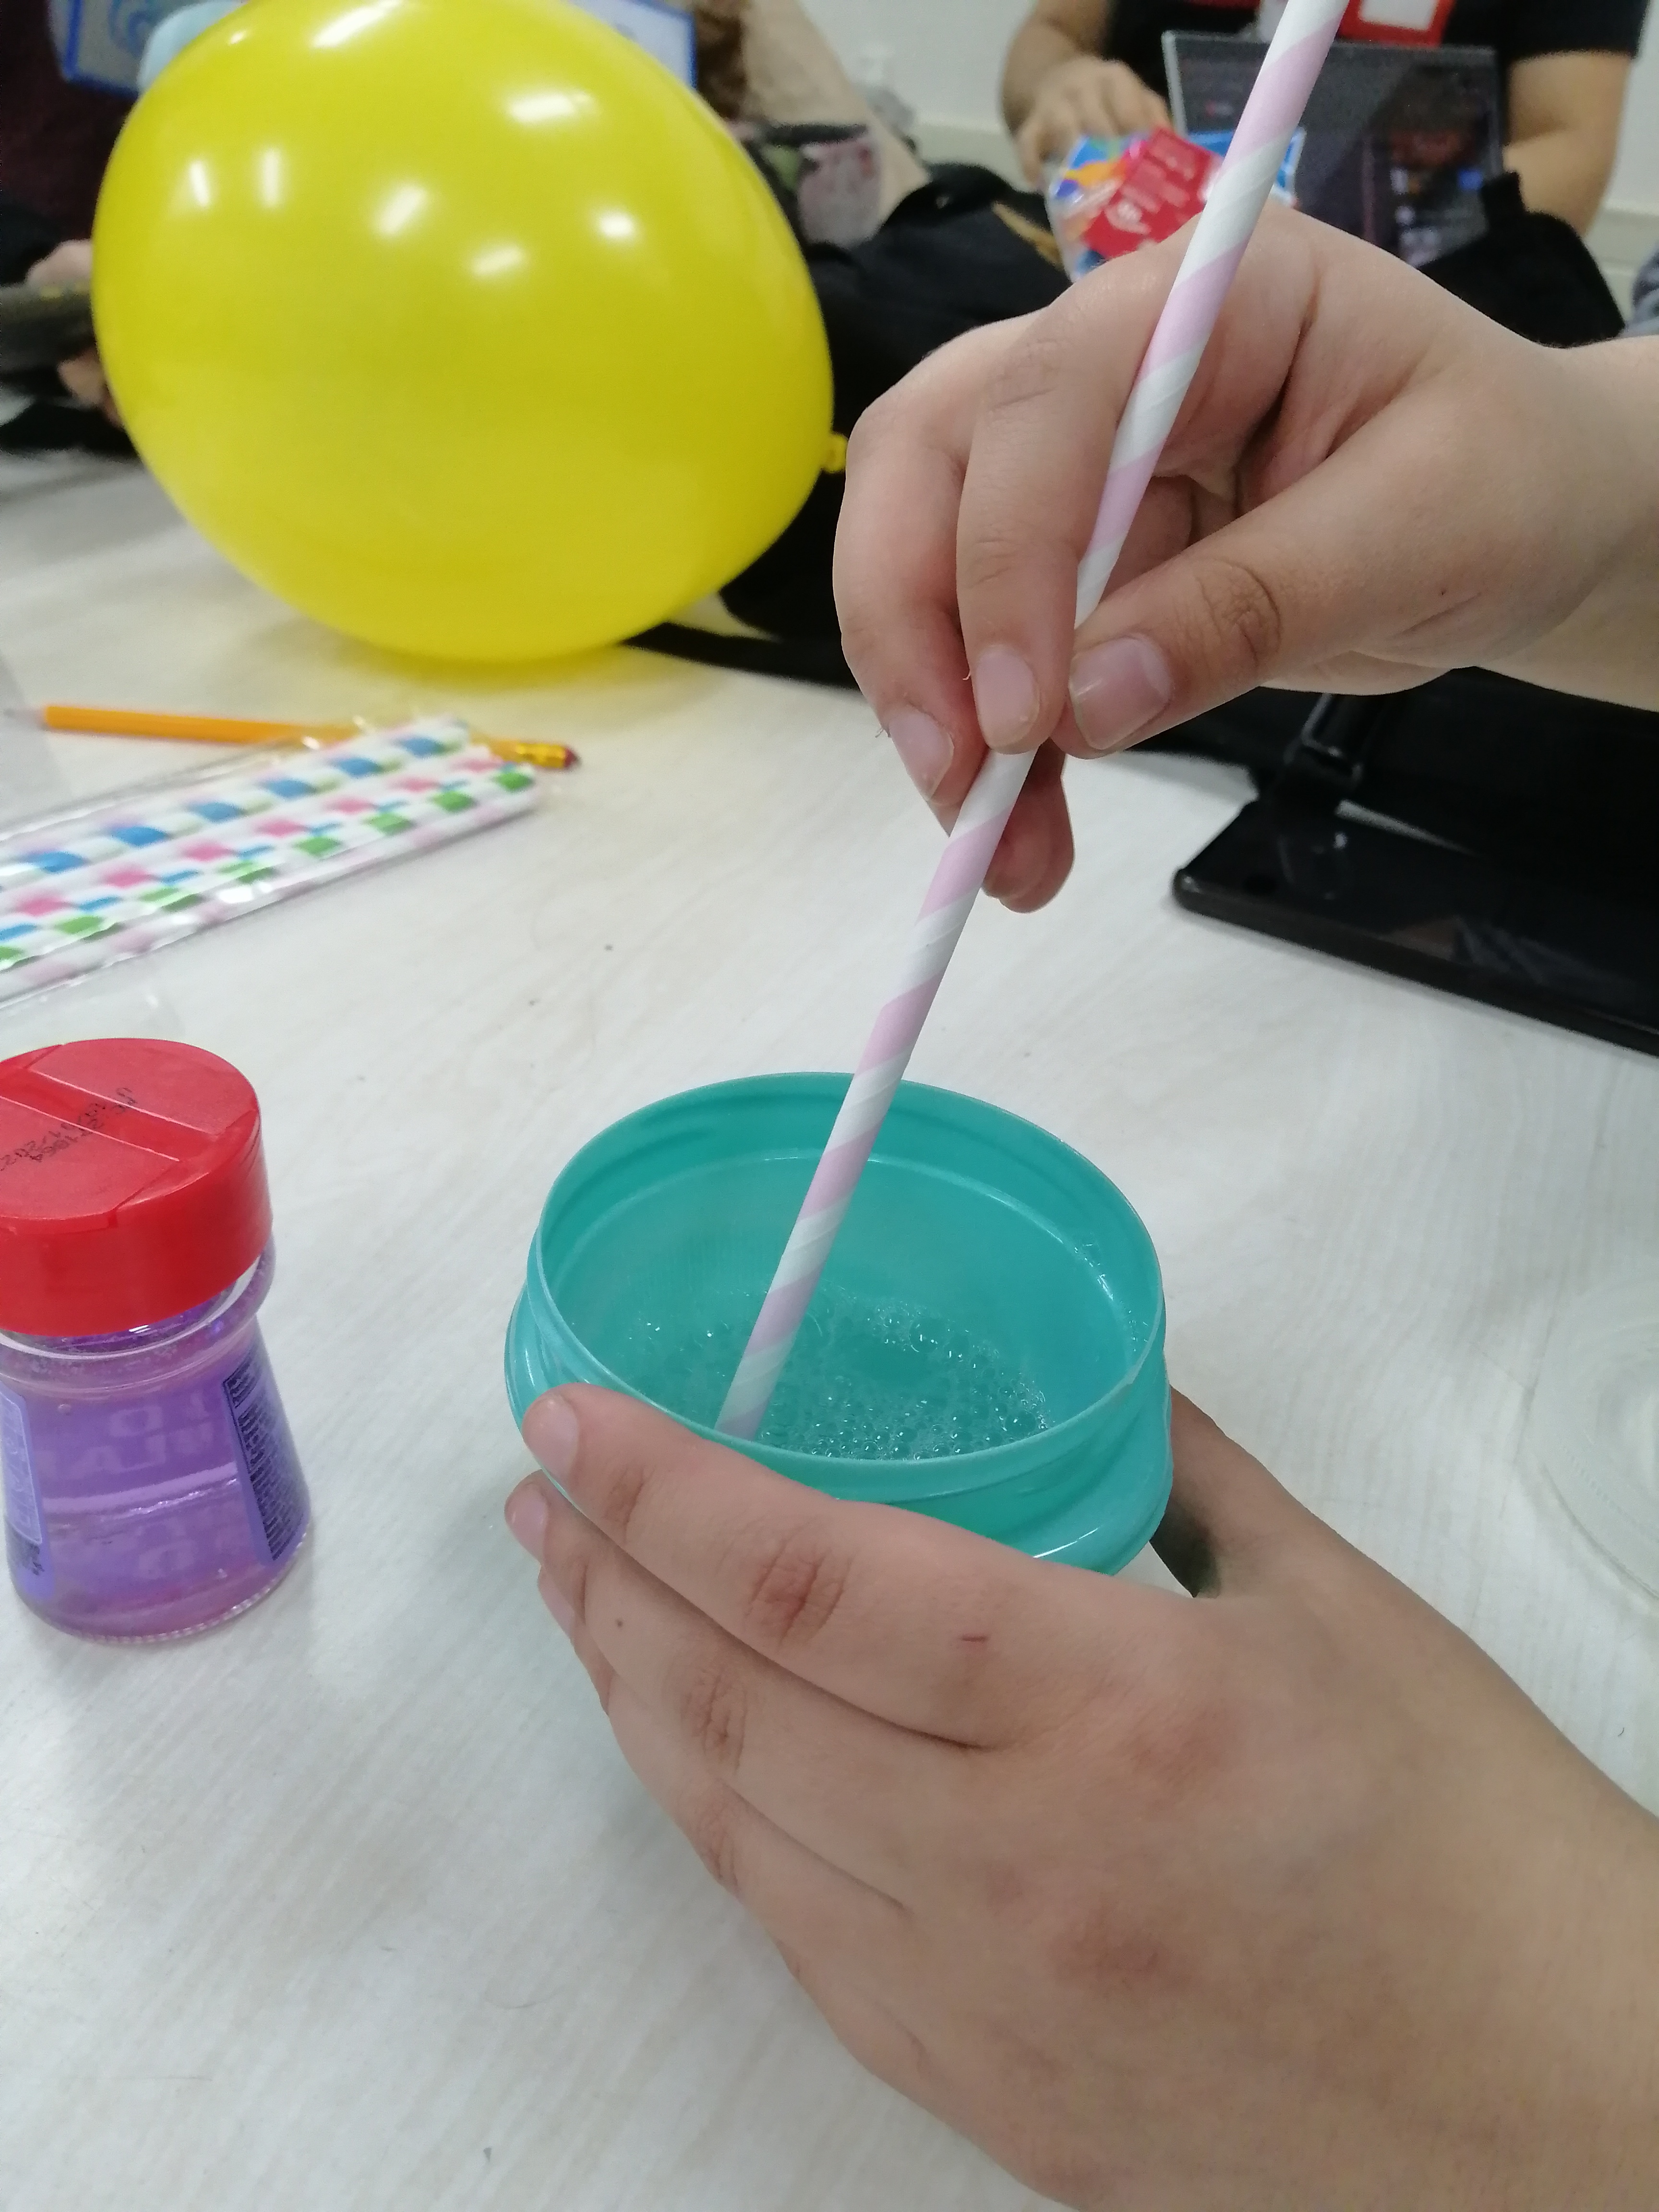
\includegraphics[width=2cm, height=3cm]{imag/Exp2_00.jpg}
    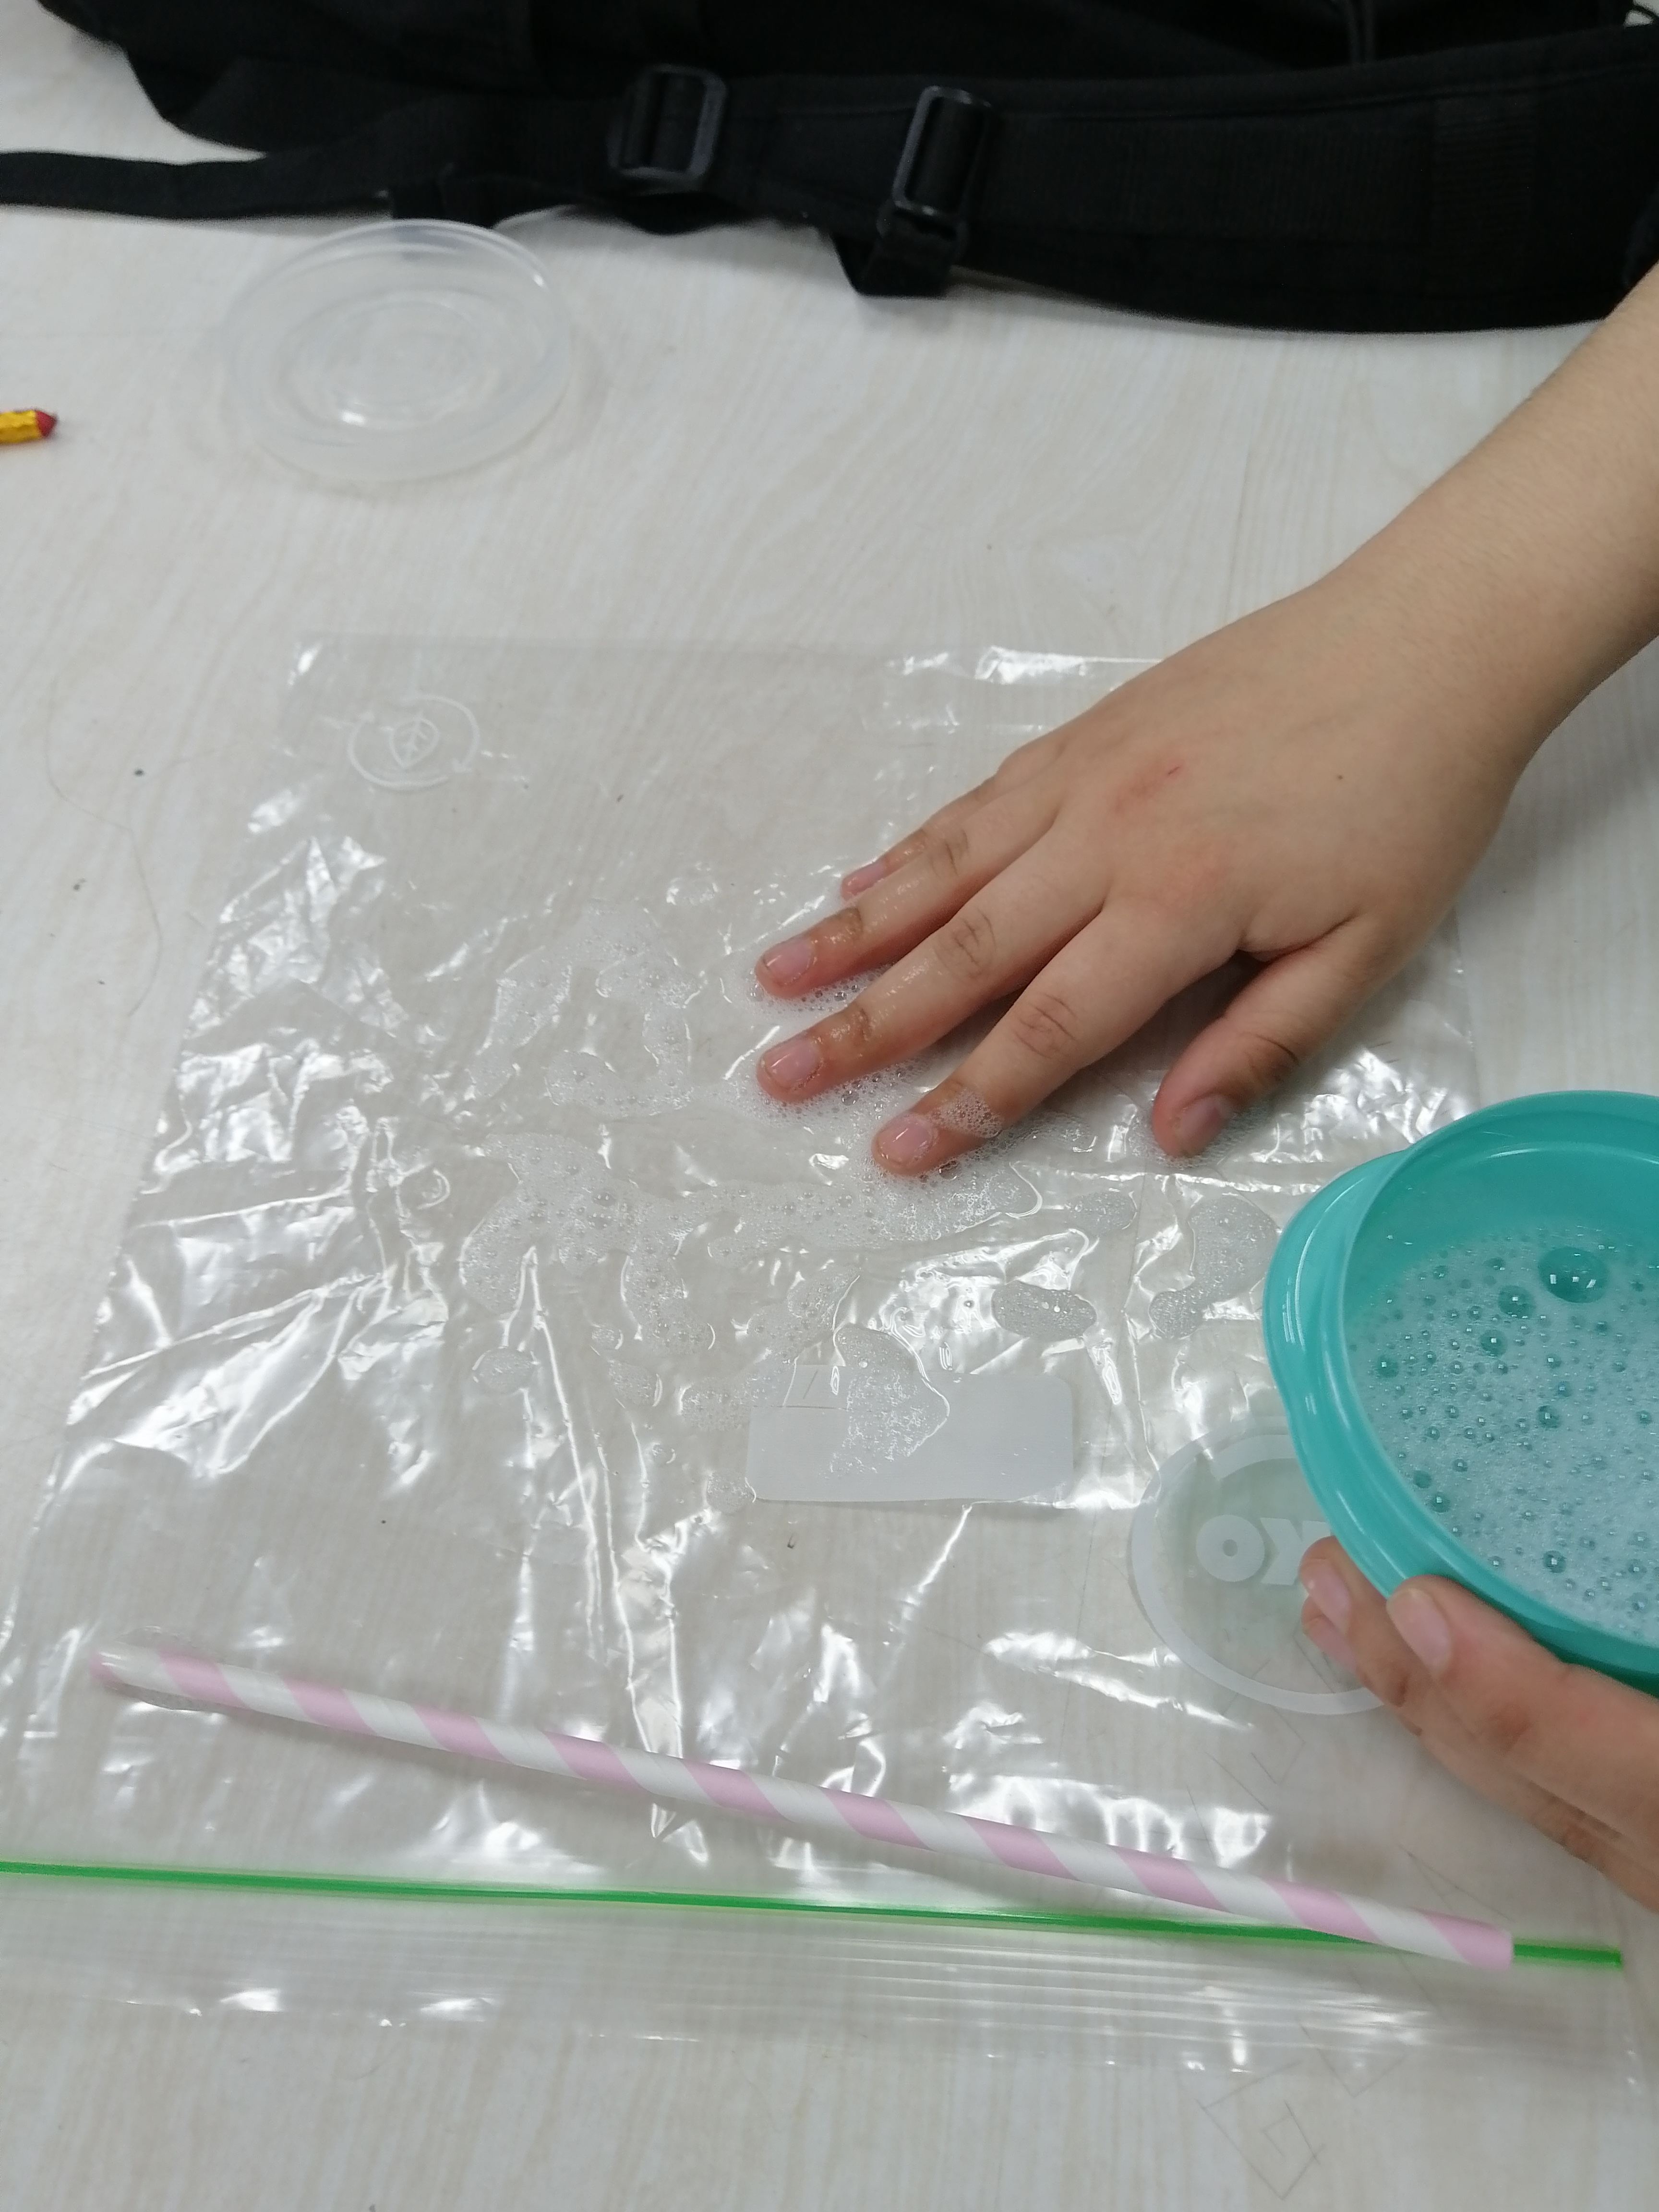
\includegraphics[width=2cm, height=3cm]{imag/Exp2_01.jpg}
    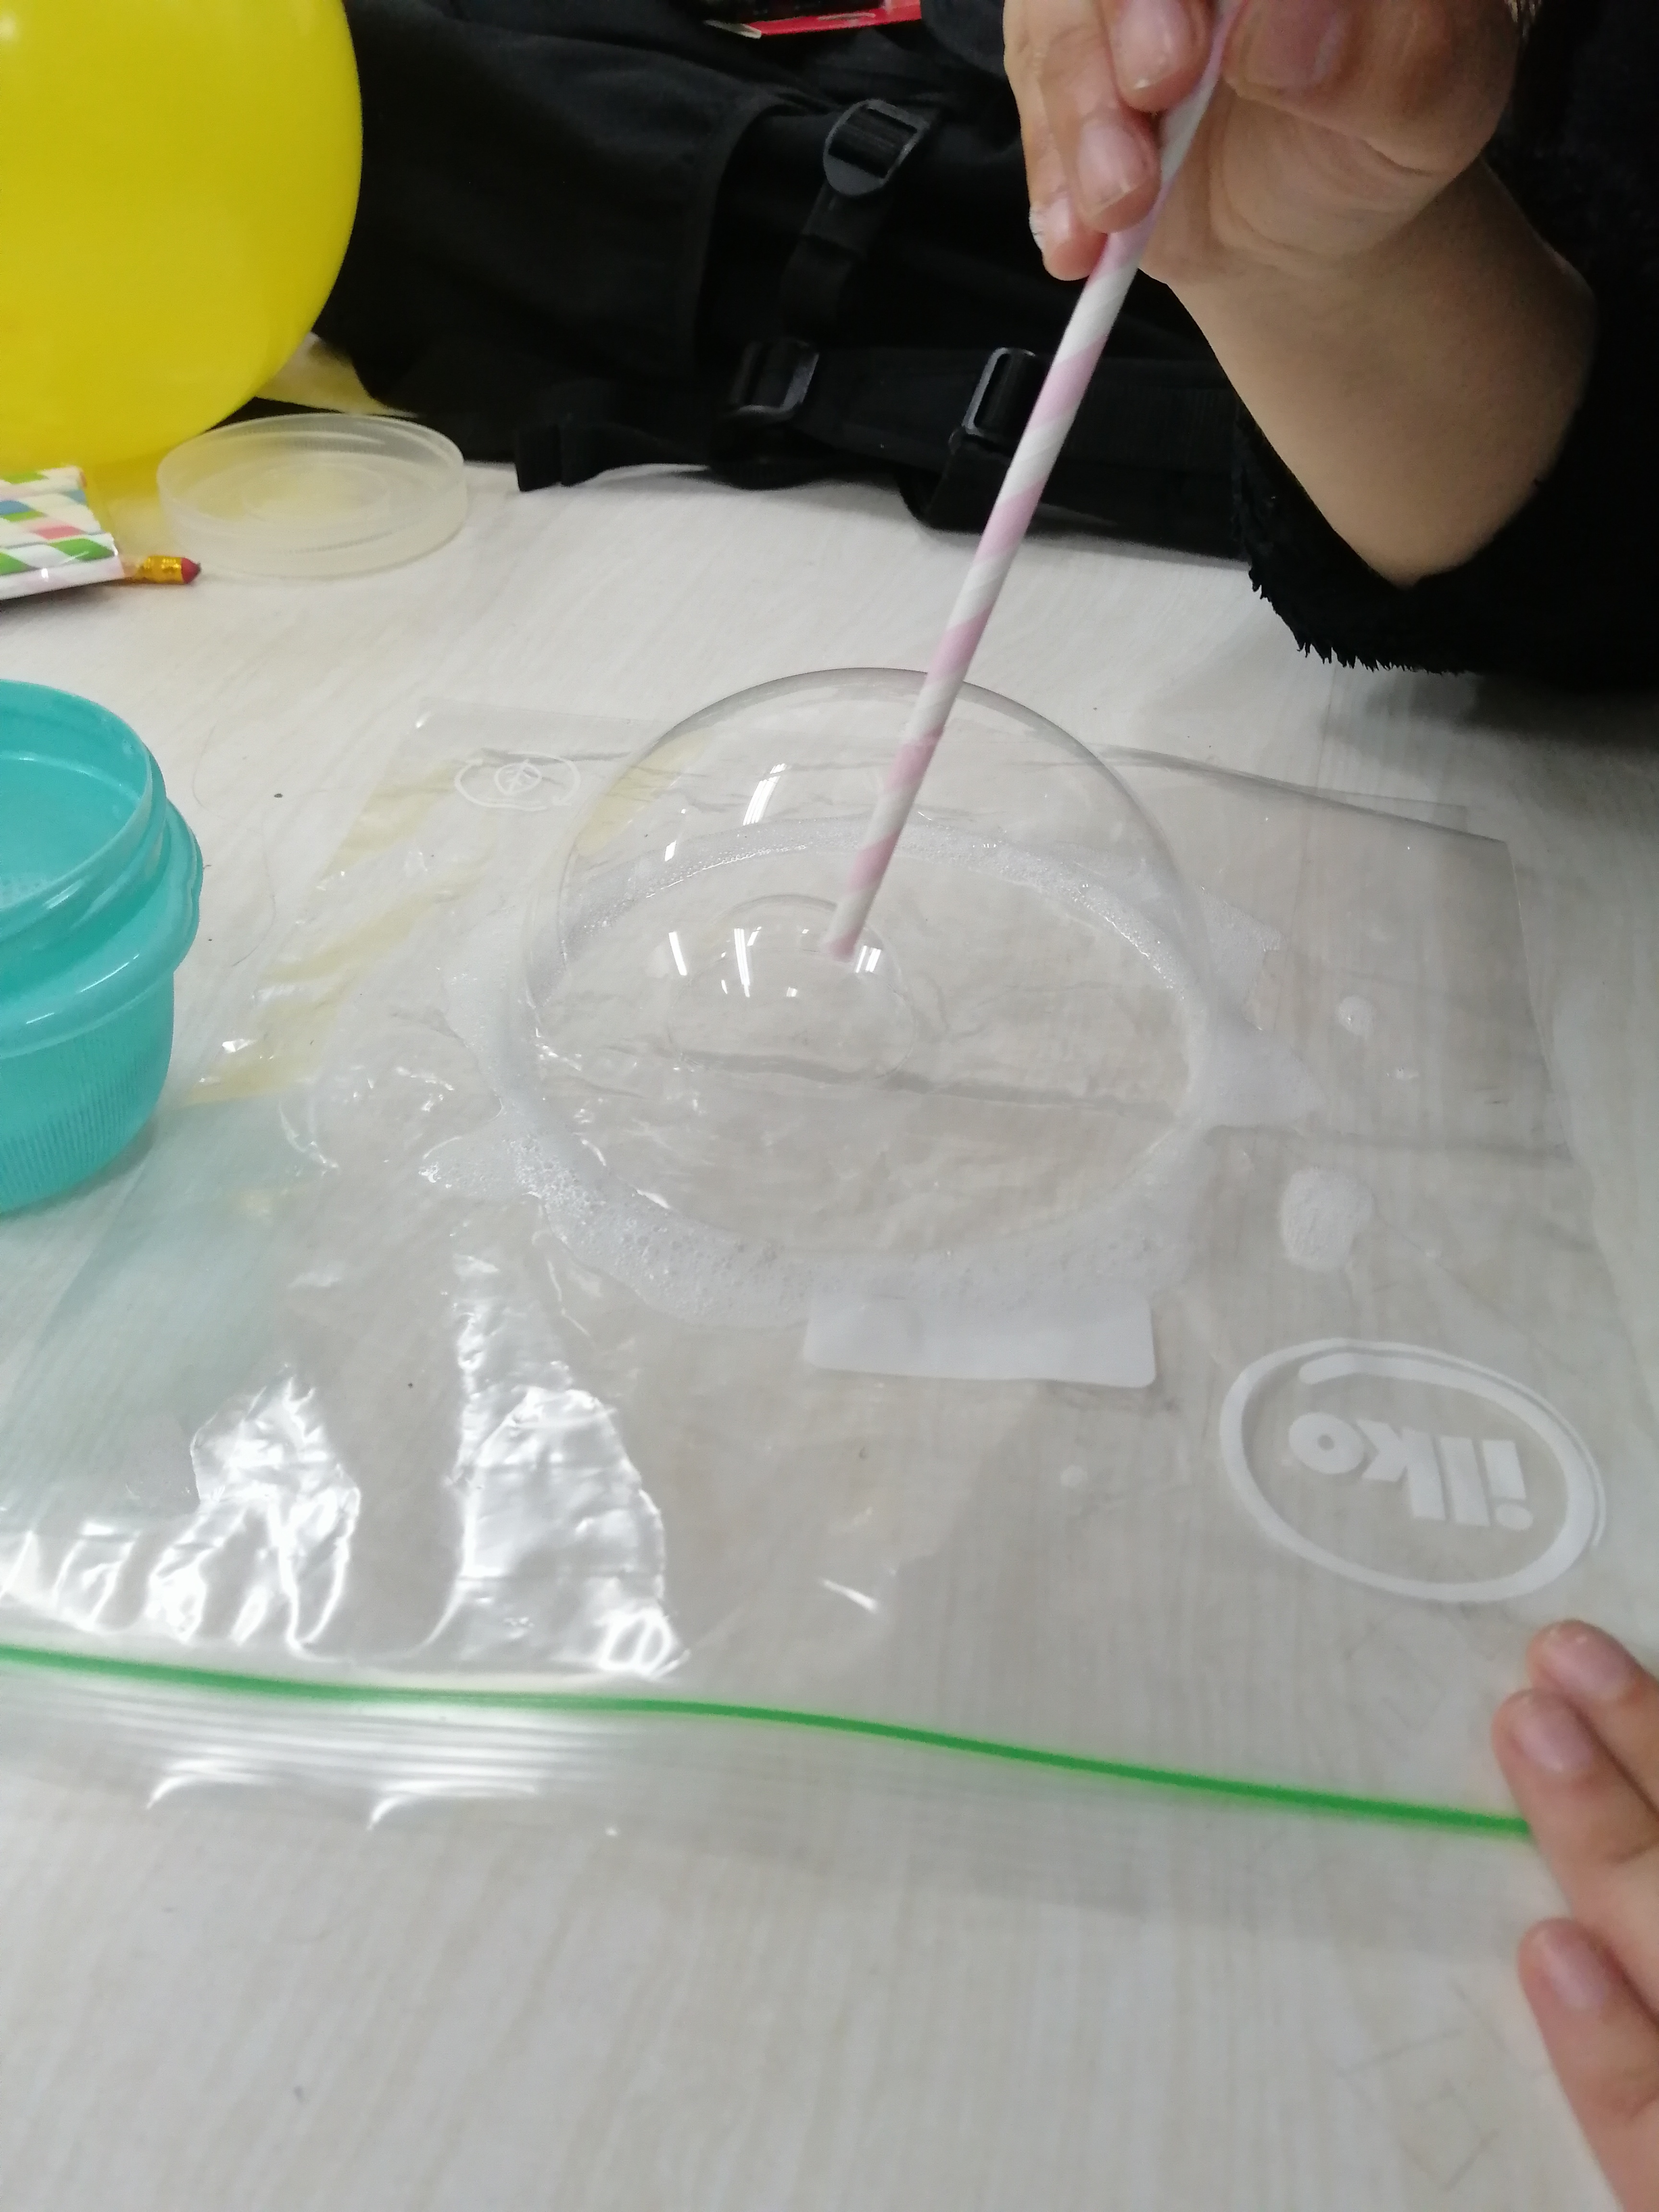
\includegraphics[width=2cm, height=3cm]{imag/Exp2_02.jpg}
\end{Figura}  

\begin{Figura}
    \centering
    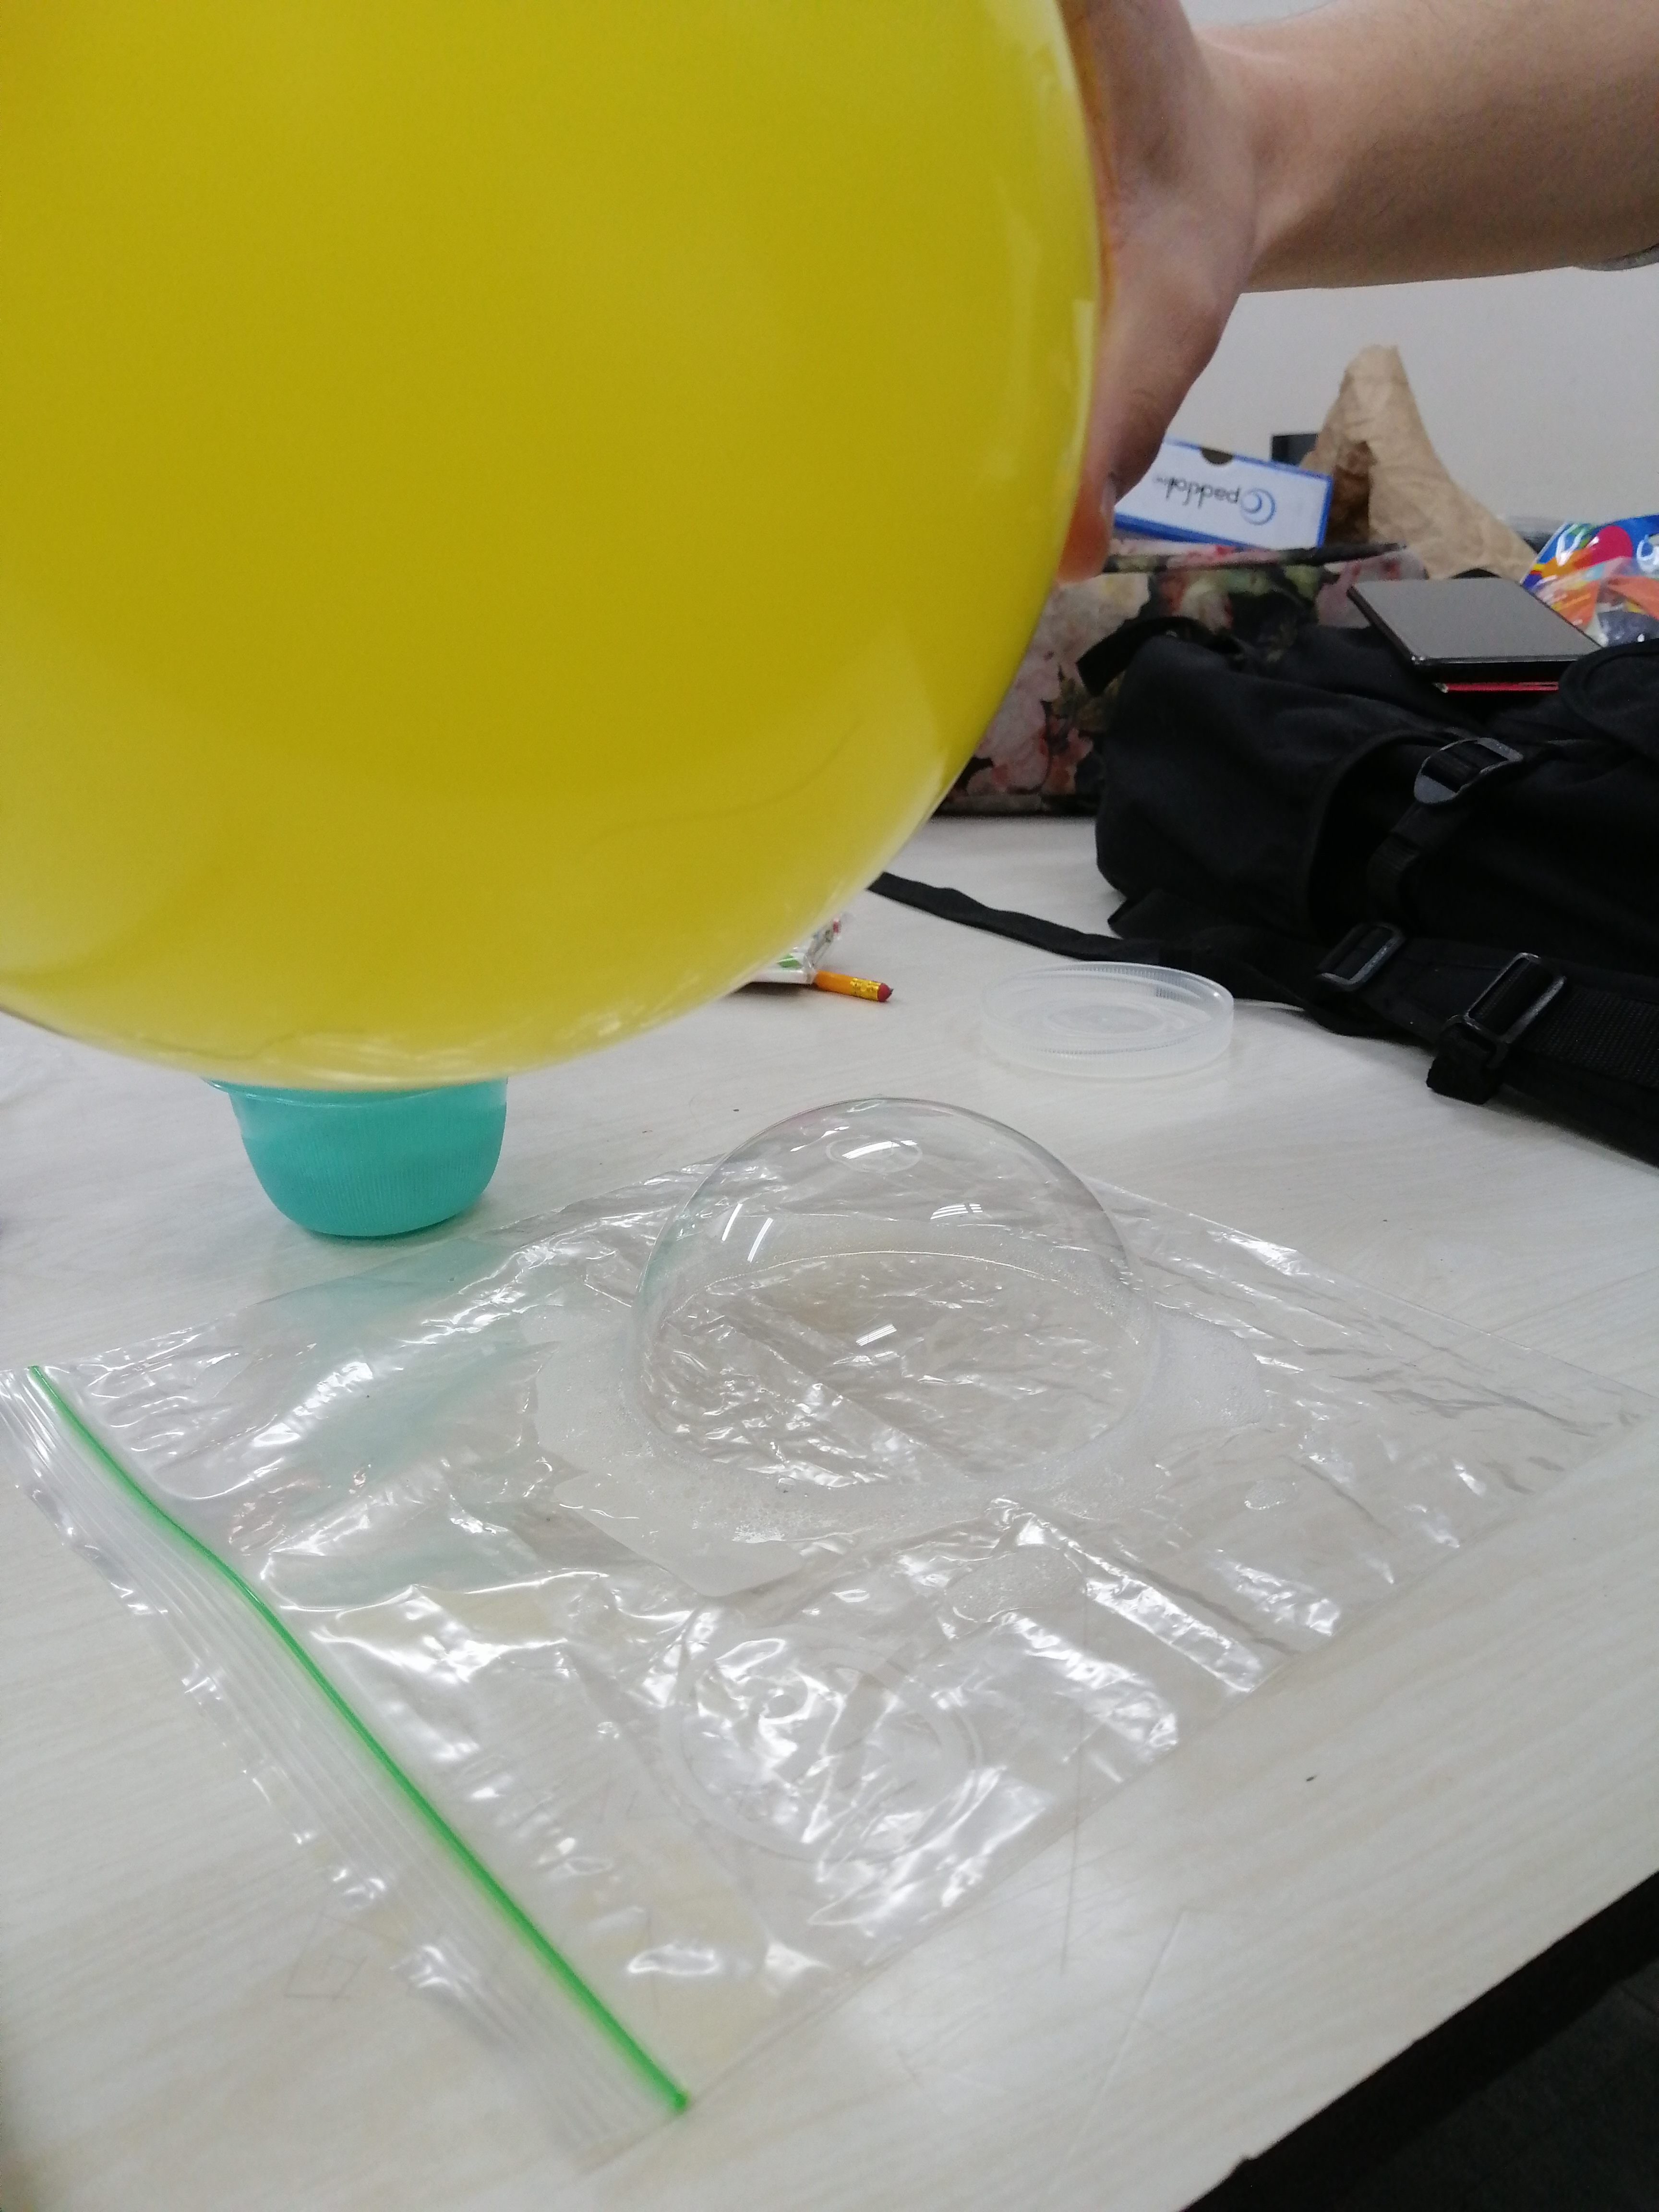
\includegraphics[width=2cm, height=3cm]{imag/Exp2_03.jpg}
    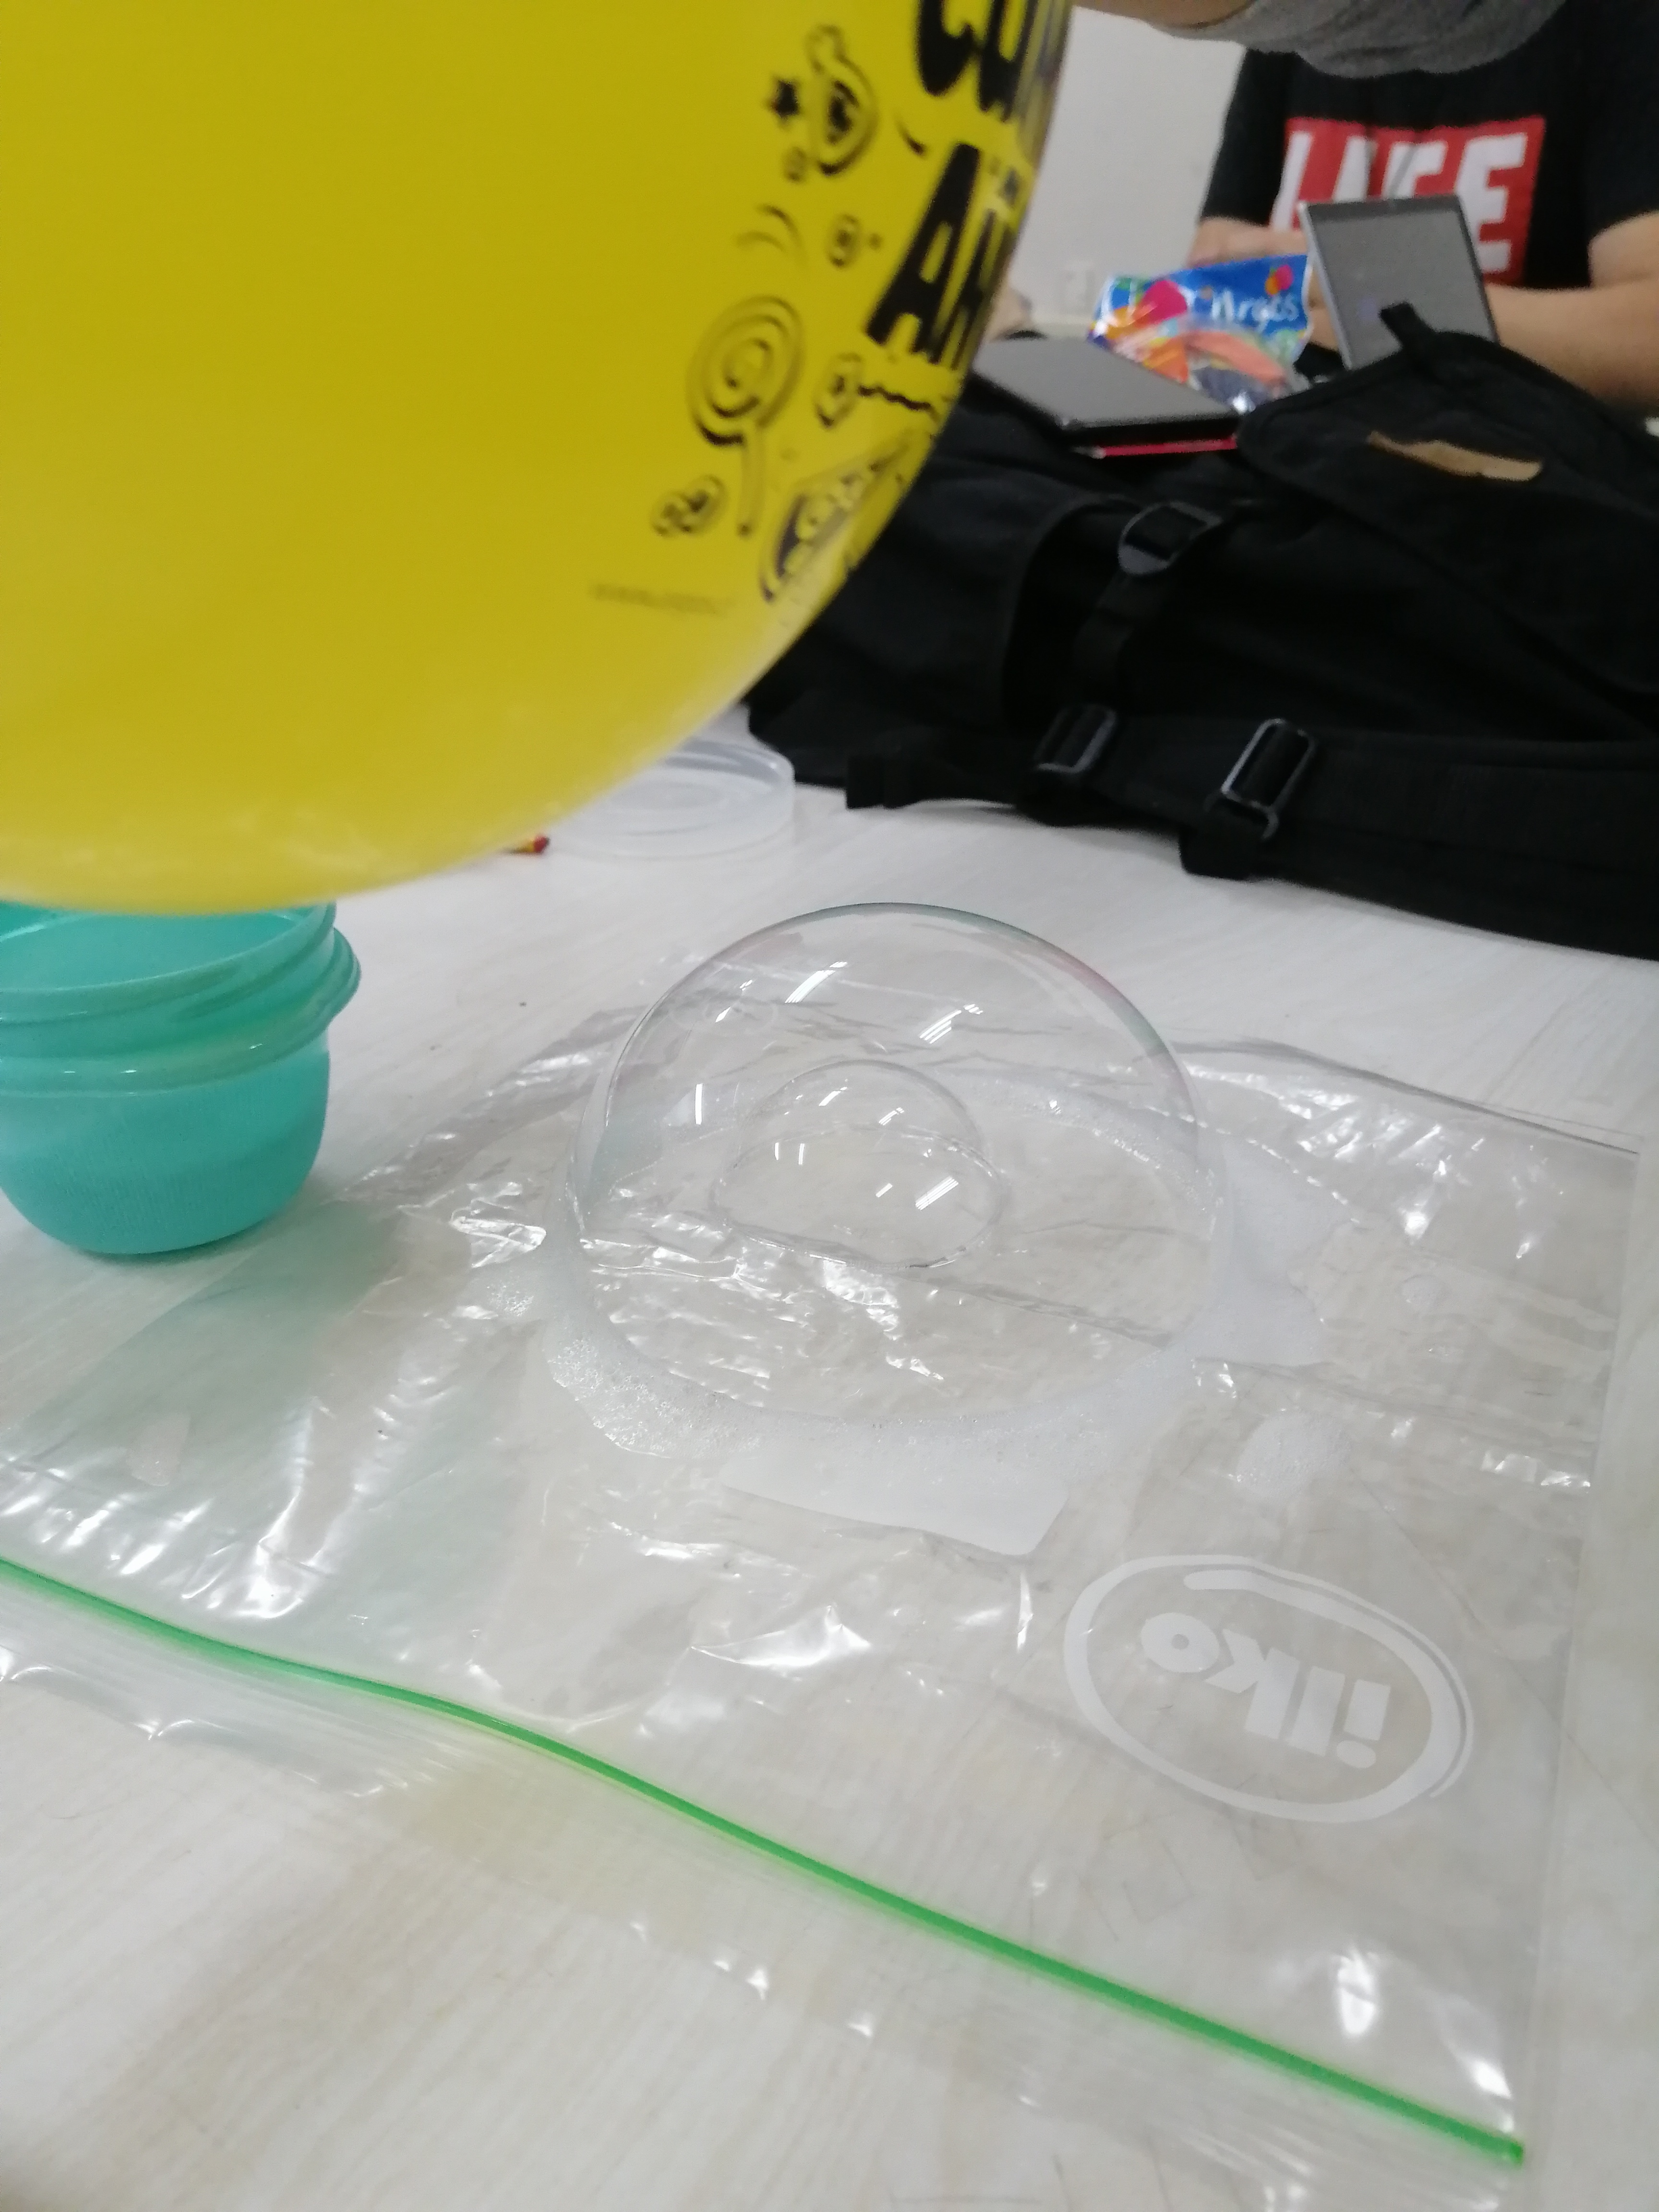
\includegraphics[width=2cm, height=3cm]{imag/Exp2_04.jpg}
\end{Figura}   




%%%%%%%%%%%%%%%%%%%%%%%%%%%%%%%%%%%%%%%%%%%%%%%%%%%%%%%%%%%%%%%%%%%%%%%

    
\section*{Experimento 3}
\textit{Materiales: Colador de metal, celular, audífonos, papel de aluminio.}
\vspace{-\topsep}
    \begin{itemize}
       \setlength{\parskip}{0pt} 
       \setlength{\itemsep}{0pt plus 1pt}
        \item Primero conectamos los audífonos al celular para utilizarlo como antena y captar las ondas de radio.
        \item Segundo, encendemos la radio del celular y comprobamos que funcione correctamente.
        \item Luego, ponemos el móvil sobre el papel de aluminio.
        \item Después, con el colador de metal, encerramos el área en donde se encuentra el celular.
        \item Observamos que el celular no percibe las ondas de radio, ya que la radio no funciona.
    \end{itemize}
\vspace{-\topsep}

%===============Imagenes================
\begin{Figura}
    \centering
    \includegraphics[width=2cm, height=3cm]{imag/Exp3_00.jpg}
    \includegraphics[width=2cm, height=3cm]{imag/Exp3_01.jpg}
\end{Figura}


    
%============Análisis=====================
\section*{Análisis}
Al ver detenidamente cada uno de los experimentos, podemos decir que guardan relación entre ellos.
En el primer experimento podemos notar que, cuando el teléfono lo envolvemos en papel de aluminio este no puede recibir llamadas ni tiener red wi-fi, esto nos quiere decir que el papel aluminio impide el paso de esas ondas electromagneticas.
En el segundo experimento podemos ver que al acercar el globo cargado de electricidad a la burbuja pequeña que está en su interior.%Falta???
En el tercer experimento podemos ver que, el papel de aluminio y el colador, crean una barrera que impide que la antena, que está formada por los audifonos conectados al celular, capte las ondas electromagnéticas, en este caso las de radio.

%En el tercer experimento podemos ver que, el papel de aluminio y el colador, crean una barrera que impide que la antena(audífonos)
%capte las ondas de radio.


%============Conclusión
\section*{Conclusión}
De lo anteriormente analizado en los 3 experimentos podemos notar que,el papel aluminio, la burbuja exterior y el colador de metal actúan como una barrera que impide el campo eléctrico, esto es porque los tres son conductores, que en presencia de un campo eléctrico alcanzan el equilibrio electroestático en la que ya no hay movimientos de cargas, porque, el campo interno del conductor se opone al campo externo aplicado sobre el, de modo que en el interior del conductor el campo se vuelve nulo \cite{Electrostatica}.La ley de Gauss explica este fenómeno, ya qué relaciona el flujo de campo eléctrico a través de cualquier superficie cerrada es igual a la carga $q$ que está encerrada dentro de la superficie, dividida por la constante de la permitividad en el vacío $\epsilon_0$.
\begin{equation}\label{eq:G}
\oint_S \! \vec{E} \cdot  \, d\vec{s} = \dfrac{q}{\epsilon_0}
\end{equation}
Por lo visto en La ley de Gauss \ref{eq:G}, al no haber carga dentro del conductor, el campo eléctrico dentro de el es nulo, lo que explica porque la burbuja pequeña y el celular no percibían las ondas electromagnéticas y eléctricas.
Con este gran descubrimiento se pudieron crear objetos capaces de apantallar las ondas electromagnéticas y volverlas más seguras ante cualquier campo demasiado intenso para nosotros los humanos , como la famosa jaula de Faraday , la cual logra evitar los daños hacia los pasajeros de un avión cuando un rayo cae sobre ellos.

%De lo anteriormente analizado en los 3 experimentos, notemos que, el papel de aluminio, la burbuja exterior y el colador de metal actúan como una barrera que impide el paso de un
%campo electrico...
%============Referencias (en APA)

\end{multicols*}



\begin{thebibliography}{5}
    \bibitem{Electrostatica}  Electrostática. Conductores en equilibrio electrostático. (s. f.). Recuperado 9 de septiembre de 2022, 
    de \url{https://www2.montes.upm.es/dptos/digfa/cfisica/electro/conductores.html}
    \bibitem{Resnick} \textbf{D. Halliday; R. Resnick; K. S. Kane.} \textit{Física Vol. 2.} (Cap.29), Compañía Editorial Continental, S.A. de C.V. 3º Edición, 1994
     \bibitem{electromagnetismo}Electromagnetismo - Concepto, aplicaciones y ejemplos. (s. f.-b). Concepto. Recuperado 9 de septiembre de 2022,
     de \url{https://concepto.de/electromagnetismo/}
    \bibitem{Jaula de Faraday}Jaula de Faraday - Qué es, cómo funciona, ejemplos y aplicaciones. (s. f.-b). Concepto. Recuperado 9 de septiembre de 2022, 
    de \url{https://concepto.de/jaula-de-faraday/}
\end{thebibliography}
























\end{document}
